\begin{figure}[!htbp]
  \centering
  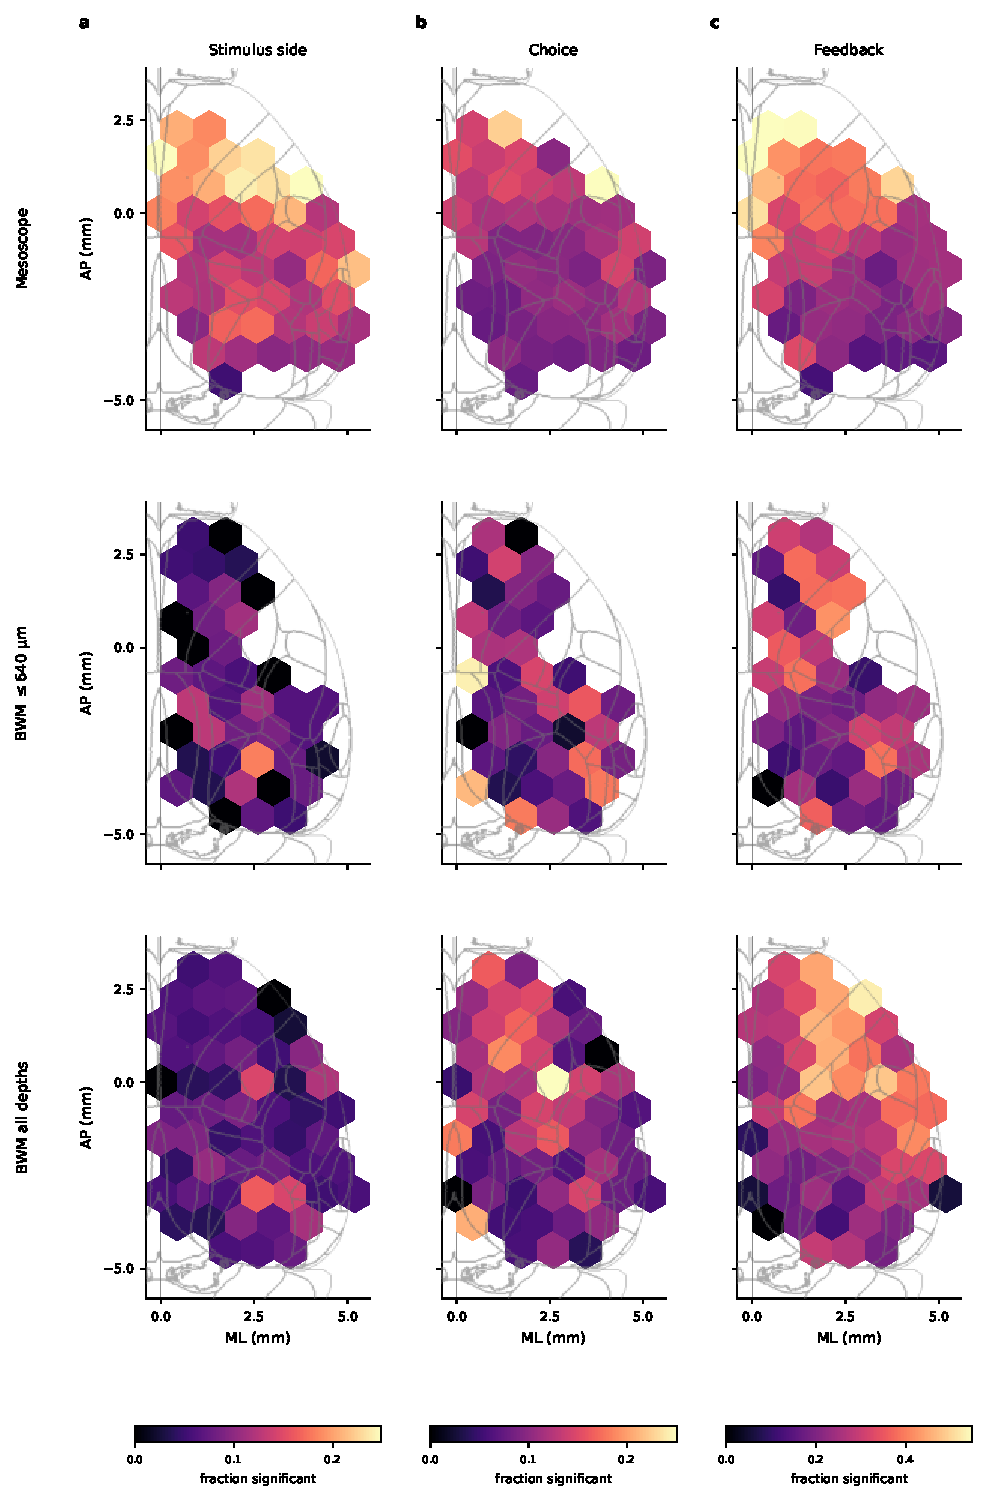
\includegraphics[width=\linewidth,height=0.8\textheight,keepaspectratio]{figures/tuning.pdf}
  \caption{Tuning results: mesoscope two-photon imaging (top row; deconvolved activity of isocortex neurons) vs Brain Wide Map Neuropixels units within 640\,$\mu$m of the pial surface (middle row; twice the depth range the mesoscope images, 174--318\,$\mu$m) and at all depths (bottom row; reference). Each neuron is assigned to a hexagonal bin (1\,mm vertex to vertex) by its ML and AP Allen CCF position; hemispheres folded onto the right. Grey lines: Allen top-view region boundaries. Colour scales are shared across rows. Single-neuron tuning: the BWM single-cell test (brainwidemap single\_cell\_stats, re-implemented on the GPU and checked against the original), applied identically to both modalities to the mean activity in each window. Mann--Whitney $U$ statistics are computed within condition strata, summed and normalised; the null distribution comes from 3000 permutations of the condition labels within consecutive blocks, and $p$ is the rank of the observed statistic. Mesoscope windows are 0.3\,s long because the frame period is about 0.2\,s. \textbf{a} Fraction of neurons per bin tuned to stimulus side ($p<0.05$; bins with $\geq$10 neurons pooled across sessions); window $[0, 0.1]$\,s (BWM) or $[0, 0.3]$\,s (mesoscope) relative to stimulus onset. \textbf{b} Choice; window $[-0.1, 0]$\,s (BWM) or $[-0.3, 0]$\,s (mesoscope) relative to movement onset. \textbf{c} Feedback; window $[0, 0.2]$\,s (BWM) or $[0, 0.3]$\,s (mesoscope) relative to feedback.}
  \label{fig:tuning}
\end{figure}
